\thispagestyle{lichsutoanhocnone}
\pagestyle{lichsutoanhoc}
\graphicspath{{../lichsutoanhoc/pic/}}
\everymath{\color{lichsutoanhoc}}
\blfootnote{$^1$\color{lichsutoanhoc}THPT chuyên Hà Nội -- Amsterdam.}
\begingroup
\AddToShipoutPicture*{\put(0,616){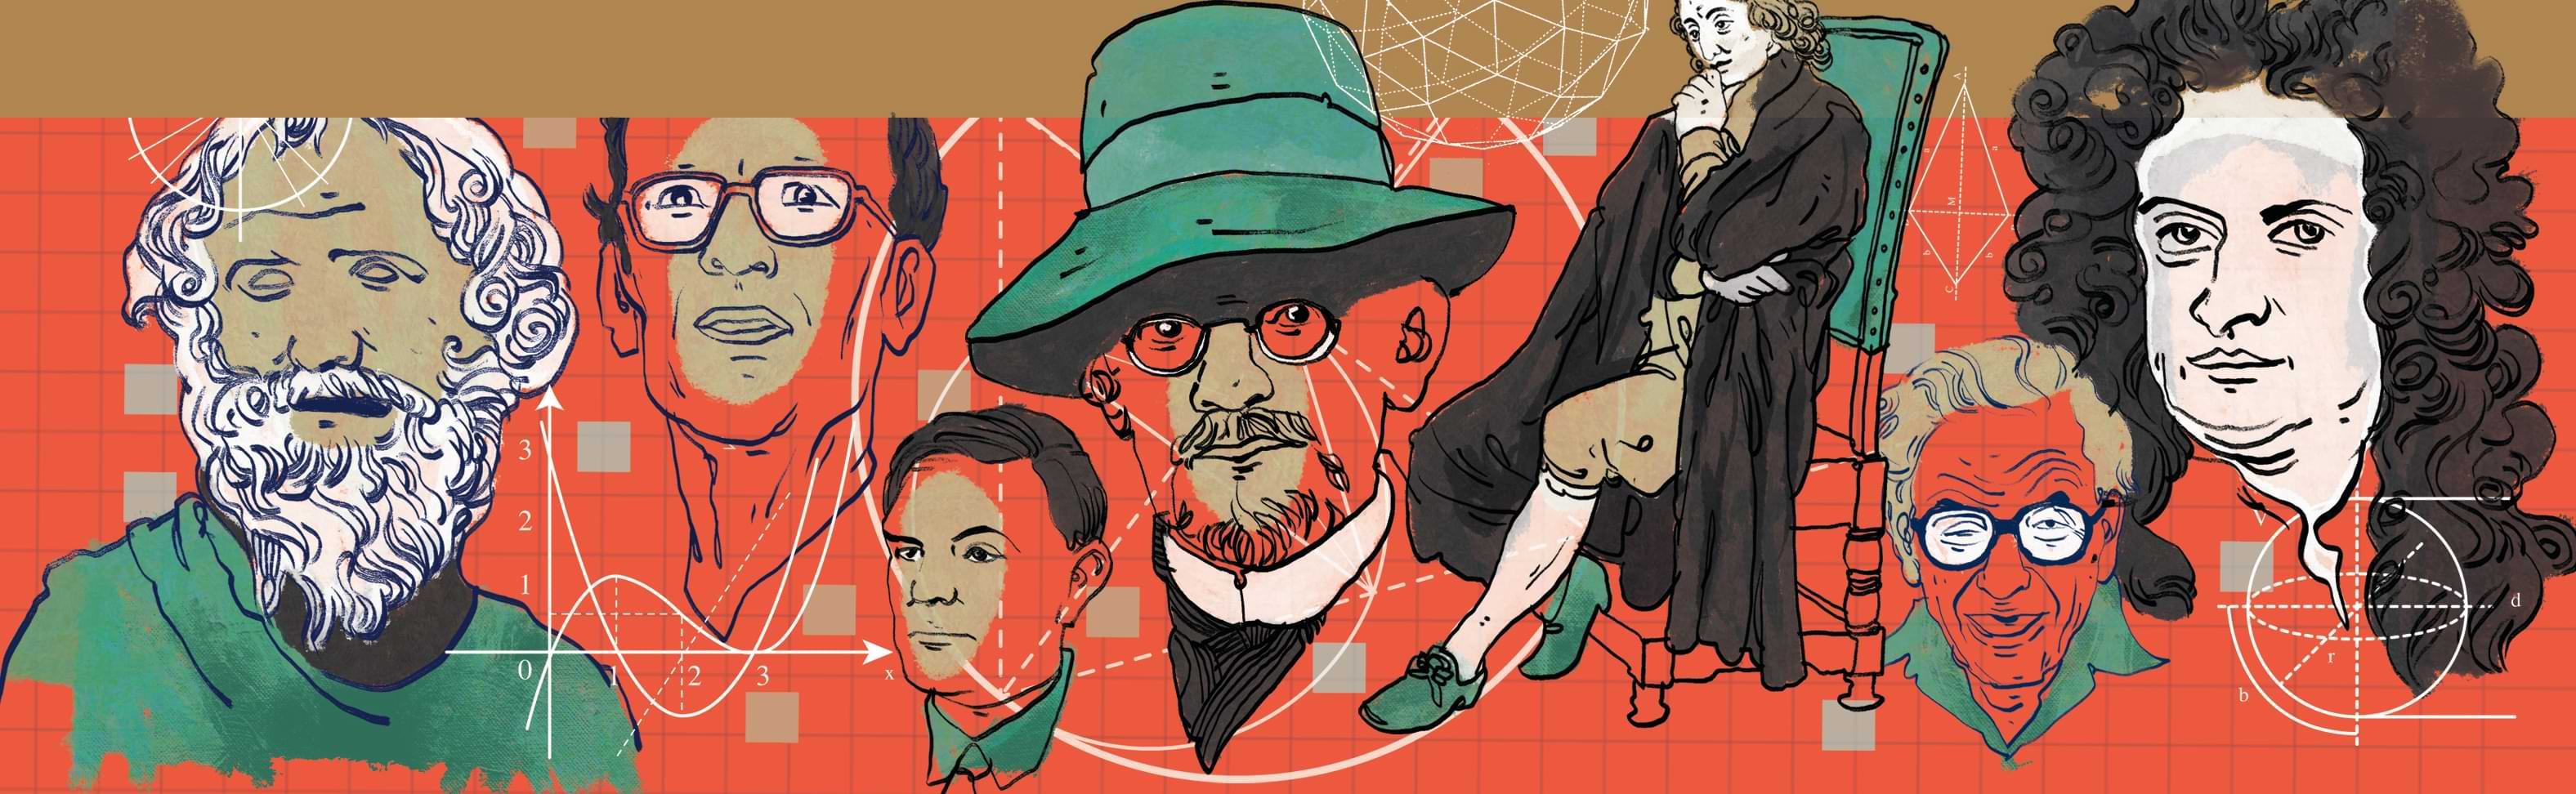
\includegraphics[width=19.3cm]{../bannerlichsu}}}
\AddToShipoutPicture*{\put(96,520){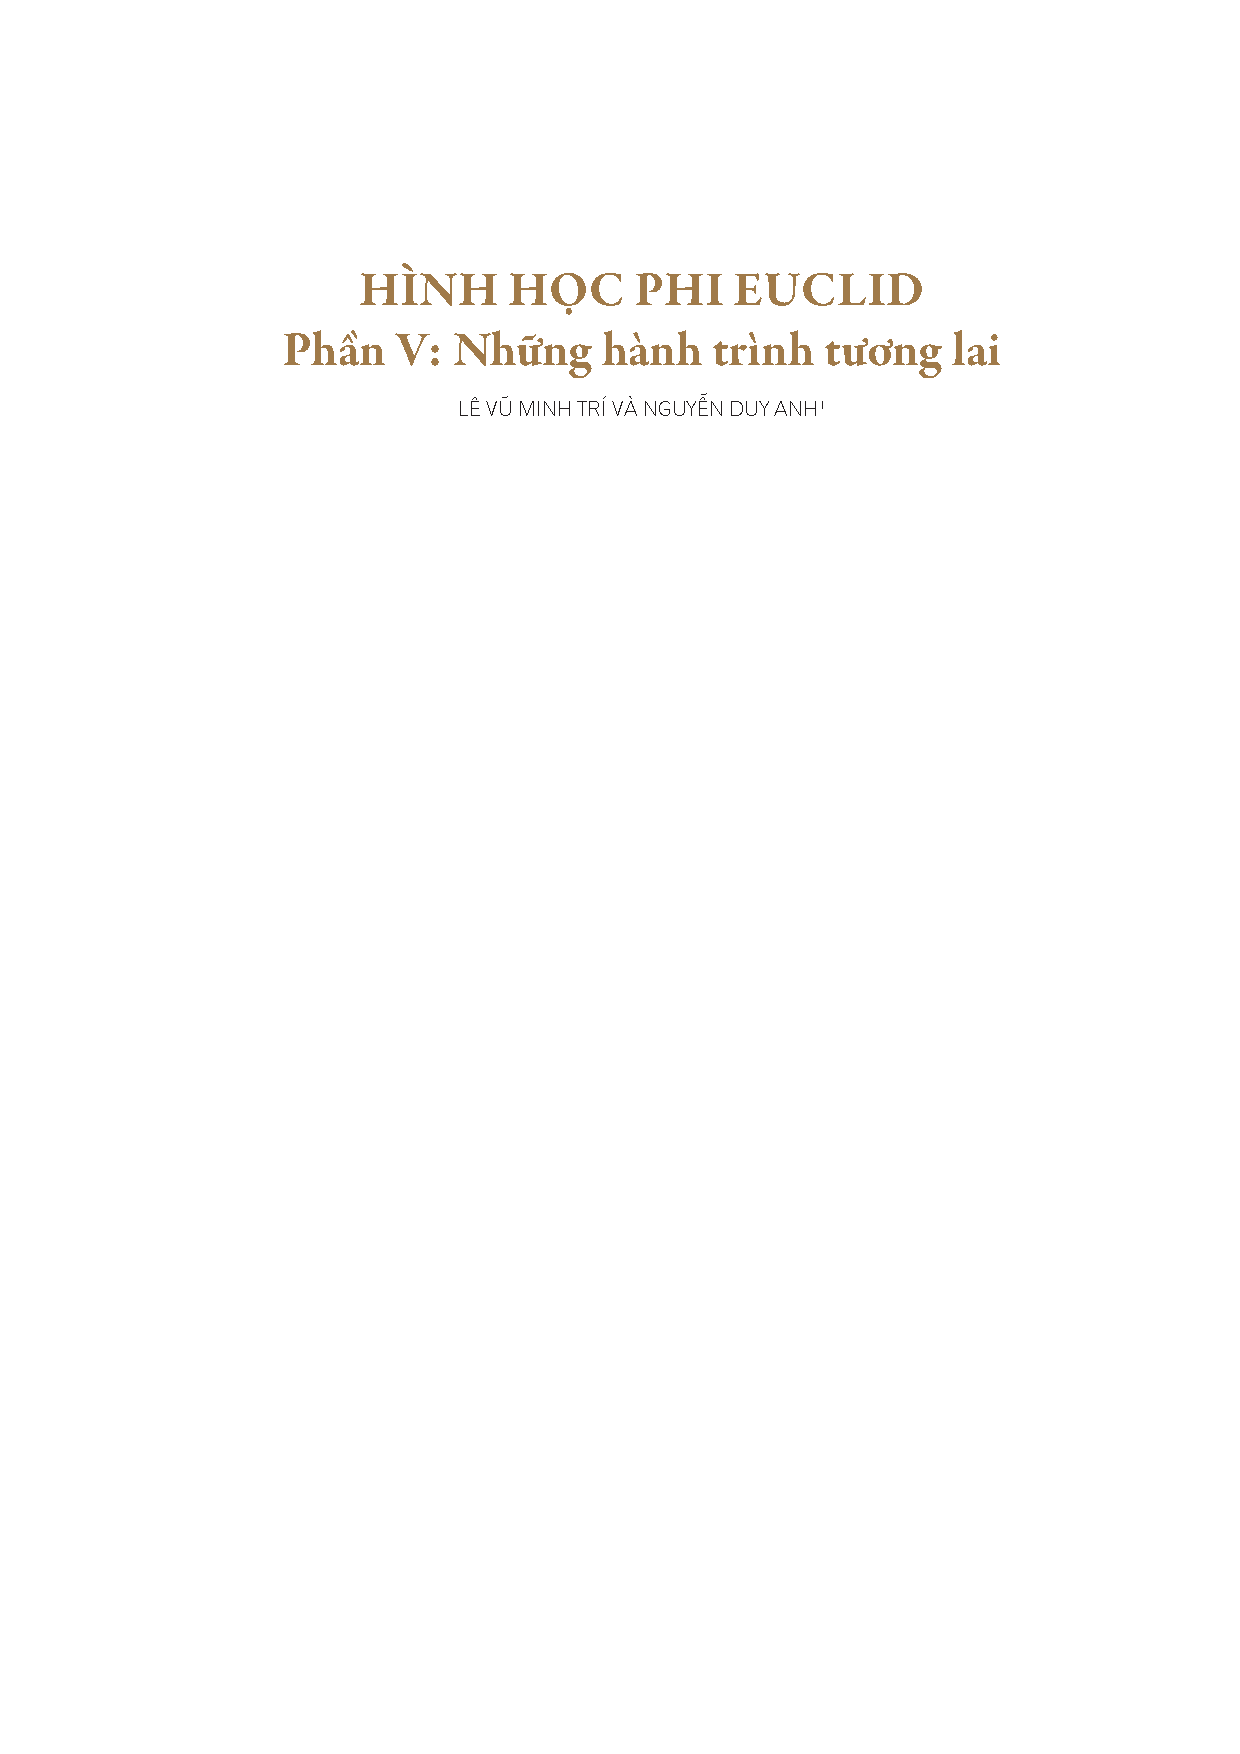
\includegraphics[scale=1]{../tieude4.pdf}}}
\centering
\endgroup

\vspace*{185pt}

\begin{multicols}{2}
	Để đảm bảo cho cuộc hành trình phía trên suôn sẻ, chúng tôi đã lược bớt một số chi tiết nhỏ để những bài viết cô đọng hơn. Bài viết này là chặng cuối của chuyến đi, cũng là một số tổng kết và những cái tên để những độc giả hứng thú có thêm nguồn tham khảo. Tất nhiên hành trình của chúng ta mới chỉ là thuật lại bước đầu chật vật khẳng định vị thế của hình học phi Euclid, và hành trình của lĩnh vực nghiên cứu này vẫn còn hết sức rộng mở phía trước.
	\vskip 0.1cm
	\textbf{\color{lichsutoanhoc}Đôi lời về các tiên đề:}
	\vskip 0.1cm
	Tiên đề không phải sự thật tự nó hiển nhiên, nó đơn thuần là luật chơi của thế giới đó. Và vì thế có hơn một hệ tiên đề diễn tả cùng loại hình học Euclid ta biết. Nổi tiếng nhất là luận án Grundlagen der Geometrie (Nền tảng của hình học) của nhà tiên phong, nhà thông thái David Hilbert $(1862-1943)$ trong một nỗ lực thống nhất các ngành toán học với nhau. Công trình với $21$ tiên đề và $6$ khái niệm nguyên thủy (Euclid đưa ra $5$ tiên đề, $0$ định nghĩa nguyên thủy) của ông có tinh thần khá tương đồng với cách phát triển của Euclid. 
	Ngoài ra ta có các đóng góp đến từ G. Peano, M. Pieri, G. Veronese, O. Veblen, G. de B. Robinson, E. V. Huntington, H. G. Forder, và G. Birkhoff. Chẳng hạn như cách lập tiên đề của Pieri chỉ có hai khái niệm nguyên thủy là ``điểm" và ``chuyển động".
	\vskip 0.1cm
	\textbf{\color{lichsutoanhoc}Hình học hyperbolic khác hình học Euclid như thế nào?}
	\vskip 0.1cm
	Công chuẩn bị của chúng ta từ đầu giờ đây sẽ có ích. Khi mà tiên đề song song đã không còn đúng, những mệnh đề tương đương với nó cũng vậy, từ ấy ta có những kết quả đáng chú ý như dưới đây. 
	Góc ở đỉnh của tứ giác Saccheri và góc thứ tư của tứ giác Lambert không phải góc vuông, mà là góc nhọn. Thậm chí hình chữ nhật còn không tồn tại trong thế giới này. Diện tích các tam giác bị chặn. Cả Bolyai và Lobachevsky đều phát hiện ra rằng diện tích tam giác trong hình học này tỉ lệ thuận với độ lệch -- hiệu của pi với tổng ba góc trong tam giác đó tính theo radian. Không tồn tại hai tam giác đồng dạng nhưng không bằng nhau nữa. Nói cách khác, hai tam giác đồng dạng thì bằng nhau. 
	\vskip 0.1cm
	Một hệ quả của điều này là chúng ta không thể định nghĩa các hàm lượng giác như trong hình học Euclid. Các hàm $\sin$, $\cos$ quen thuộc giờ được định nghĩa thông qua chuỗi lũy thừa Đồng thời có hai hàm hyperbolic hữu ích mà người ta cũng nghiên cứu ở đây là $\sinh$ và $\cosh$, có chuỗi lũy thừa giống của $\sin$ và $\cos$ bỏ đi $(-1)^n$, hay viết gọn lại thông qua hàm mũ cơ số $e$: 
	\begin{align*}
		&\cos(x) =  1 - \frac{x^2}{2!} + \frac{x^4}{4!} - ... \\
		&\sin(x) =  x - \frac{x^3}{3!} + \frac{x^5}{5!} - ... \\
		&\cosh(x) =  1 + \frac{x^2}{2!} + \frac{x^4}{4!} + ... \\
		&\sinh(x) =  x + \frac{x^3}{3!} + \frac{x^4}{4!} - ... 
	\end{align*}
	Giờ đây không phải có một mà là hai đường gọi là đường song song giới hạn (limiting parallel). Cụ thể, với điểm $P$ và đường thẳng $l$ không đi qua nó, sẽ tồn tại hai đường thẳng $d_1, d_2$ đối xứng nhau qua đường vuông góc $d$ hạ từ $P$ xuống $l$. Hai đường này là hai đường tạo với $d$ góc nhỏ nhất mà song song với $l$. 
	\vskip 0.1cm
	Và cuối cùng, hằng số $\pi$  không thể được định nghĩa như ở hình Euclid, bởi chu vi của đường tròn chia cho bán kính của nó trong không gian này còn chẳng phải một tỉ số cố định. Những điều trông rất hợp lý trong hình học Euclid, chẳng hạn như tỉ lệ giữa chu vi và bán kính của mọi đường tròn là như nhau, lại không đúng ở đây. Trong không gian hình học hyperbolic độ cong $-1$, chu vi của đường tròn bán kính $r$ được tính theo công thức: $C = 2\pi\cdot\sinh r$. 
	\vskip 0.1cm
	\textbf{\color{lichsutoanhoc}Hình học elliptic khác hình học Euclid như thế nào?}
	\vskip 0.1cm
	Theo cách thiết lập tiên đề theo hướng của Euclid, ta sẽ không thể thay thế được tiên đề $5$ bằng ``mọi đường thẳng đều cắt nhau" ngay. Bởi kết hợp định lý $16$ và $27$ thì ta thấy là đường song song tồn tại. Mặt khác, nhìn vào mô hình nửa mặt cầu của mặt phẳng elliptic ta đã dựng, việc một điểm nằm giữa hai điểm khác trông hơi sai sai, vì ``đường thẳng" ở mô hình này trông như những đường tròn. Vì thế các tiên đề về sự nằm giữa sẽ được thay thế bằng các tiên đề về sự phân cách (separation axiom). Một số điểm khác biệt so với hình học Euclid của hình học elliptic cũng tương tự như với hình học hyperbolic. Trong hình học elliptic, diện tích của một tam giác sẽ bị chặn và tỉ lệ thuận với hiệu của tổng ba góc tam giác đó (vẫn theo radian) với $\pi$, hai góc ở đỉnh của tứ giác Saccheri và góc thứ tư của tứ giác Lambert đều là góc tù. Không còn những tam giác đồng dạng nhưng không bằng nhau, vì thế hàm lượng giác cứ phải định nghĩa bằng chuỗi lũy thừa. Tất nhiên đây sẽ còn là một thế giới xa lạ với ta hơn cả hình hyperbolic, bởi cả quan hệ nằm giữa đã cần sửa thành sự phân tách để các tiên đề không dẫm vào chân nhau.
	\vskip 0.1cm
	\textbf{\color{lichsutoanhoc}Đóng góp của Riemann và di sản của hành trình}
	\vskip 0.1cm
	Những ý tưởng mà Bolyai và Lobachevsky đã thúc đẩy là khá mới mẻ với giới tri thức đương thời. Dù vậy, thời gian đã dần xua tan những nghi ngờ còn sót lại của đại đa số học giả. Người ta dần học được vài điều. Những tiên đề không phải là chân lý hay sự thật vĩnh cửu, chúng chỉ là những quy ước con người đề ra. Khi thay đổi các tiên đề thì ta sẽ tạo ra các hệ thống kết quả khác nhau, chúng ta sẽ không nghi ngờ liệu nó có đúng trong thực tế hay không, mà sẽ đi vào phát triển những hệ thống cho ra những kết quả thú vị, hoặc để tìm ra một mâu thuẫn nào đó để bác bỏ hệ thống đó.
	\vskip 0.1cm
	Như đã hứa, ta cùng quay ngược thời gian về ngày $10/6/1854$, Gottingen. Trong căn phòng nơi bài Habilitation lecture diễn ra, hầu hết các thính giả đều không hiểu gì mấy, thậm chí cả trưởng khoa Toán ngồi nghe còn có phần lúng túng. Bài nói chuyện là về Hình học, nhưng trên bảng không có lấy một hình vẽ nào. Phải đến $10$ năm sau giới Toán học mới dần vỡ ra ý nghĩa của những gì diễn ra ngày hôm ấy: đến tận 1868 những nội dung được bàn luận mới được đưa ra rộng rãi. Riêng việc bài nói vượt xa kỳ vọng của trưởng khoa Gauss thôi đã chứng thực cho sự kỳ tài của giảng viên trẻ Bernhard Riemann rồi. Và bởi vì đi sâu vào chi tiết còn hơi quá tầm với cả những thính giả hôm ấy, chúng ta sẽ chỉ đi qua những ý tưởng chính Riemann đã phát triển, bắt đầu với khái niệm độ cong.
	\vskip 0.1cm
	Đầu tiên, xét một đường cong bất kỳ trên mặt phẳng Euclid. Với một điểm $P$ nằm trên đường cong, cho hai điểm $Q$, $R$ tiến dần về $P$, khi đó đường tròn ngoại tiếp tam giác $PQR$ sẽ có giới hạn là đường tròn mật tiếp của đường cong tại $P$. Nếu đường tròn đó có bán kính $r$, thì độ cong của đường cong đó tại $P$ sẽ là $k = 1/r$ hoặc $k =  -(1/r)$, tùy vào việc đường tròn đó nằm về phía nào so với đường cong.
	\vskip 0.1cm
	Tiếp theo ta đến với đường cong bất kỳ trong không gian ba chiều. Đường tròn mật tiếp khi này nằm trên mặt phẳng Pi nào đó (ta gọi là mặt phẳng mật tiếp), và độ cong $k$ giờ trở thành một vectơ tại $P$, hướng về tâm đường tròn mật tiếp, độ lớn $1/r$
	\vskip 0.1cm
	Giờ ta đến với một bề mặt $S$ bất kỳ trong không gian ba chiều. Trong trường hợp này, một bề mặt được gọi là có thể định hướng được nếu nó có hai mặt, mỗi mặt hướng về một phía khác nhau. Cho dễ hiểu: Một tờ giấy là một mặt phẳng định hướng được, còn một dải Mobius thì không. Giả sử $S$ định hướng được. Nếu $d$ là một đường cong trên $S$, thì ở mỗi điểm $P$ trên gamma ta định nghĩa được một độ cong $k$.
	\vskip 0.1cm
	Gọi đường thẳng đi qua $P$, vuông góc với mặt phẳng tiếp tuyến tại $P$ là $N$. Xét một mặt phẳng chứa $N$ nào đó. Giao tuyến của mặt phẳng đó với $S$ là một đường cong (nằm trên mặt). Mỗi đường cong này có một độ cong khác nhau tại điểm $P$. Euler đã chứng minh những độ cong khác nhau này có giá trị lớn nhất và giá trị nhỏ nhất. Hai đường cong tương ứng với hai giá trị này được gọi là các đường cong chính (principle curve), và Euler chứng minh được hai đường cong chính sẽ vuông góc với nhau nếu chúng phân biệt. Tích độ cong của hai đường cong này được gọi là độ cong Gauss. 
	\begin{figure}[H]
		\vspace*{5pt}
		\centering
		\captionsetup{labelformat= empty, justification=centering}
		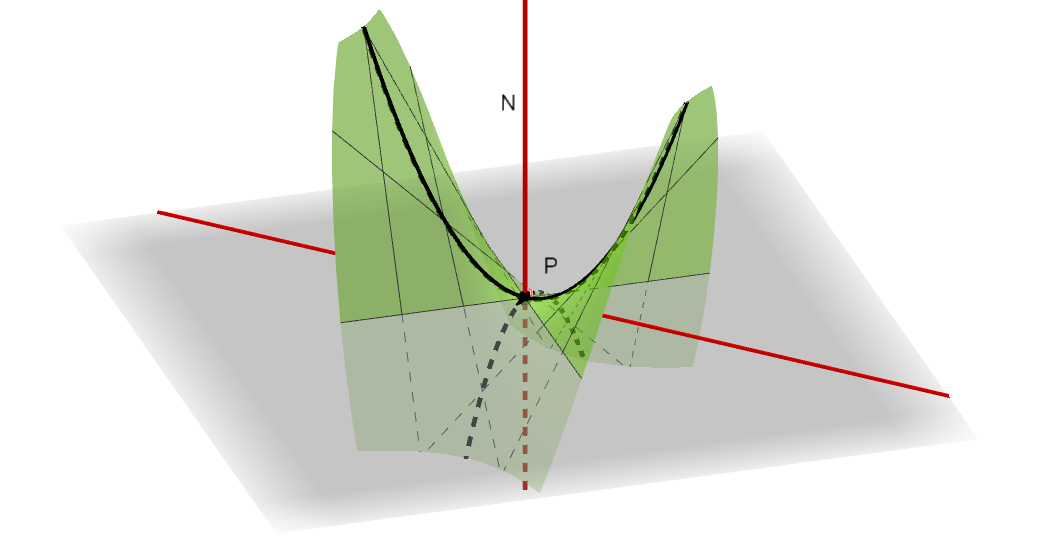
\includegraphics[width= 1\linewidth]{saddle point and riemann curvature.png}
		\caption{\small\textit{\color{lichsutoanhoc}Hai đường cong chính được tô màu đen trên hình. Nguồn: Greenberg}}
		\vspace*{-10pt}
	\end{figure}
	Gauss đã chứng minh được rằng độ cong Gauss K không thay đổi khi các bề mặt bị ``bẻ cong", miễn là sự bẻ cong ấy không thay đổi độ dài địa phương của cung và góc của những đường cong trên bề mặt ấy. 
	\vskip 0.1cm
	Ý tưởng này, cùng với ý tưởng về khoảng cách tổng quát trong các chiều không gian cao hơn và trên các bề mặt không tuân theo các tiên đề của Euclid, chính là cơ sở cho những không gian phi Euclid tổng quát hơn, và cả một lý thuyết Vật lý quan trọng nhất nhì thế kỉ hai mươi.
	\vskip 0.1cm
	$60$ năm sau bài nói chuyện vượt thời gian của Riemann tại Gottingen, một lý thuyết mới đã làm khuynh đảo Vật Lý đương thời -- Thuyết Tương đối của Einstein. Thuyết Tương đối rộng còn chỉ ra rằng thời gian và không gian có thể bị cong dựa vào khối lượng vật chất tại một vị trí. Vì vậy, hình học của lý thuyết ấy, hóa ra, lại chẳng phải hình Euclid, mà là hình học mà những Bolyai, Lobachevsky và Riemann phát triển. Một cách kiểm chứng rực rỡ cho những gì những con người tiên phong ấy đã viết nên.
	\vskip 0.1cm
	\textbf{\color{lichsutoanhoc}Tài liệu tham khảo}
	\vskip 0.1cm
	[$1$] E.T.  Bell, \textit{Men of Mathematics The Lives and Achievements of the Great Mathematicians from Zeno to Poincaré}.   
	\vskip 0.1cm
	[$2$] David M. Burton. \textit{The History of Mathematics An Introduction}. 
	\vskip 0.1cm
	[$3$] M. J. Greenberg, \textit{Euclidean and Non-Euclidean Geometries - Development and History}. 
	\vskip 0.1cm
	[$4$] Wikipedia tiếng Anh.
	\vskip 0.1cm
	[$5$] \url{https://www.youtube.com/playlist?list}\\
	\url{=PLjLK2cYtt-VBSBtvfhxx-DW3Zw3nOQ}\\ \url{HVZ}
	\vskip 0.1cm
	[$6$] \url{https://rosetta.vn/lequanganh/wp-cont} \url{ent/uploads/sites/7/2018/07/Riemann.pdf}
	\vskip 0.1cm
	[$7$] \url{https://www.cut-the-knot.org/triangle/}\\
	\url{pythpar/Drama.shtml}
\end{multicols}